% !TEX encoding = UTF-8 Unicode
\documentclass[a4paper]{report}
\usepackage{tikz}
\usepackage[margin=2.5cm]{geometry}
\usepackage{hyperref}
\usepackage{graphicx}
\usepackage{parskip}
\graphicspath{{figures/}{anotherFigureDirectory/}}
\graphicspath{ {./images/} }
\usepackage{listings}
\usepackage{wrapfig}
\usepackage{float}
\usepackage{color}
\usepackage[school,simplified]{pgf-umlcd}
\definecolor{bluekeywords}{rgb}{0.13,0.13,1}
\definecolor{greencomments}{rgb}{0,0.5,0}
\definecolor{turqusnumbers}{rgb}{0.17,0.57,0.69}
\definecolor{redstrings}{rgb}{0.5,0,0}
\definecolor{gray}{rgb}{0.13,0.13,0.13}
\lstdefinelanguage{FSharp}
                {morekeywords={let, new, match, with, rec, open, module,
                namespace, type, of, member, and, for, in, do, begin, end, fun,
                function, try, mutable, if, then, else},
                keywordstyle=\color{bluekeywords},
                sensitive=false,
                numbers=left,  % where to put the line-numbers;(none, left, right)
                numberstyle=\tiny\color{gray},
                morecomment=[l][\color{greencomments}]{///},
                morecomment=[l][\color{greencomments}]{//},
                morecomment=[s][\color{greencomments}]{{(*}{*)}},
                morestring=[b]",
                showstringspaces=false,
                stringstyle=\color{redstrings}
                }

\title{PoP - Ugeopgave 11}
\author{Christoffer, Inge og Pernille}
\date{\today}

\begin{document}
\maketitle
\tikzstyle{block} = [rectangle, draw, fill=blue!20, text centered,
    rounded corners, minimum height=2.5em]
\tikzstyle{cloud} = [rectangle, draw, fill=white, text centered,
    rounded corners, minimum height = 2em]
\tikzstyle{line} = [draw, -latex]

\section*{Preface}
As a part of our first semester course in Programming and Problem Solving, we, three budding computer scientists have improved a chess game. We've used the multi paradigm programming language Fsharp (F\#), to code our entire OO environment.


\section*{Introduction}
Chess is a game know most anywhere in the world. It's a tactical and sophisticate game dating back to 600 CE.\url{https://www.chess.com/article/view/the-history-of-chess} \href{https://www.chess.com/article/view/the-history-of-chess}{(\textsf{"History of Chess: The Basics"})}.

Many people have both failed and excelled in not only playing the game but also in creating their version and design of the game.
In this assignment we have done a mere attempt to create an application mastering a very simple version of the ancient game.


\section*{Problem analysis \& design}
The main problem with the improved chess game was to make sure that the king could not move to a square that was an available move for an opponent piece. We considered many approaches to solve this problem.
Our first approach was to use the already implemented functionality of the getVacantNNeighbours, which returned a list of available moves and which opponent pieces that could be killed in a move. We
would then use this list og available kills to check if an available move would cause an opponent piece to have a king as a kill. We decided not to do this as it was going to slow down the game. We decided to
check if the kings available moves were the same as the opponent kings available moves and if they are we then removed them as available moves. To check if there was a collision of the available moves with the rook we
decided to check if one of the coordinates of the kings avialable moves was also one of the coordinates of the rook.


DET HAR VI IKKE VÆRET SUPER GODE TIL AT SKRIVE TIDLIGERE, VI HAR SLET IKKE TIDLIGERE SKREVET OM LØSNINGSMULIGHEDER, SÅ DET TÆNKER JEG ER DET VI FOKUSERER PÅ AT SKRIVE LIDT OM.


\subsection*{UML}
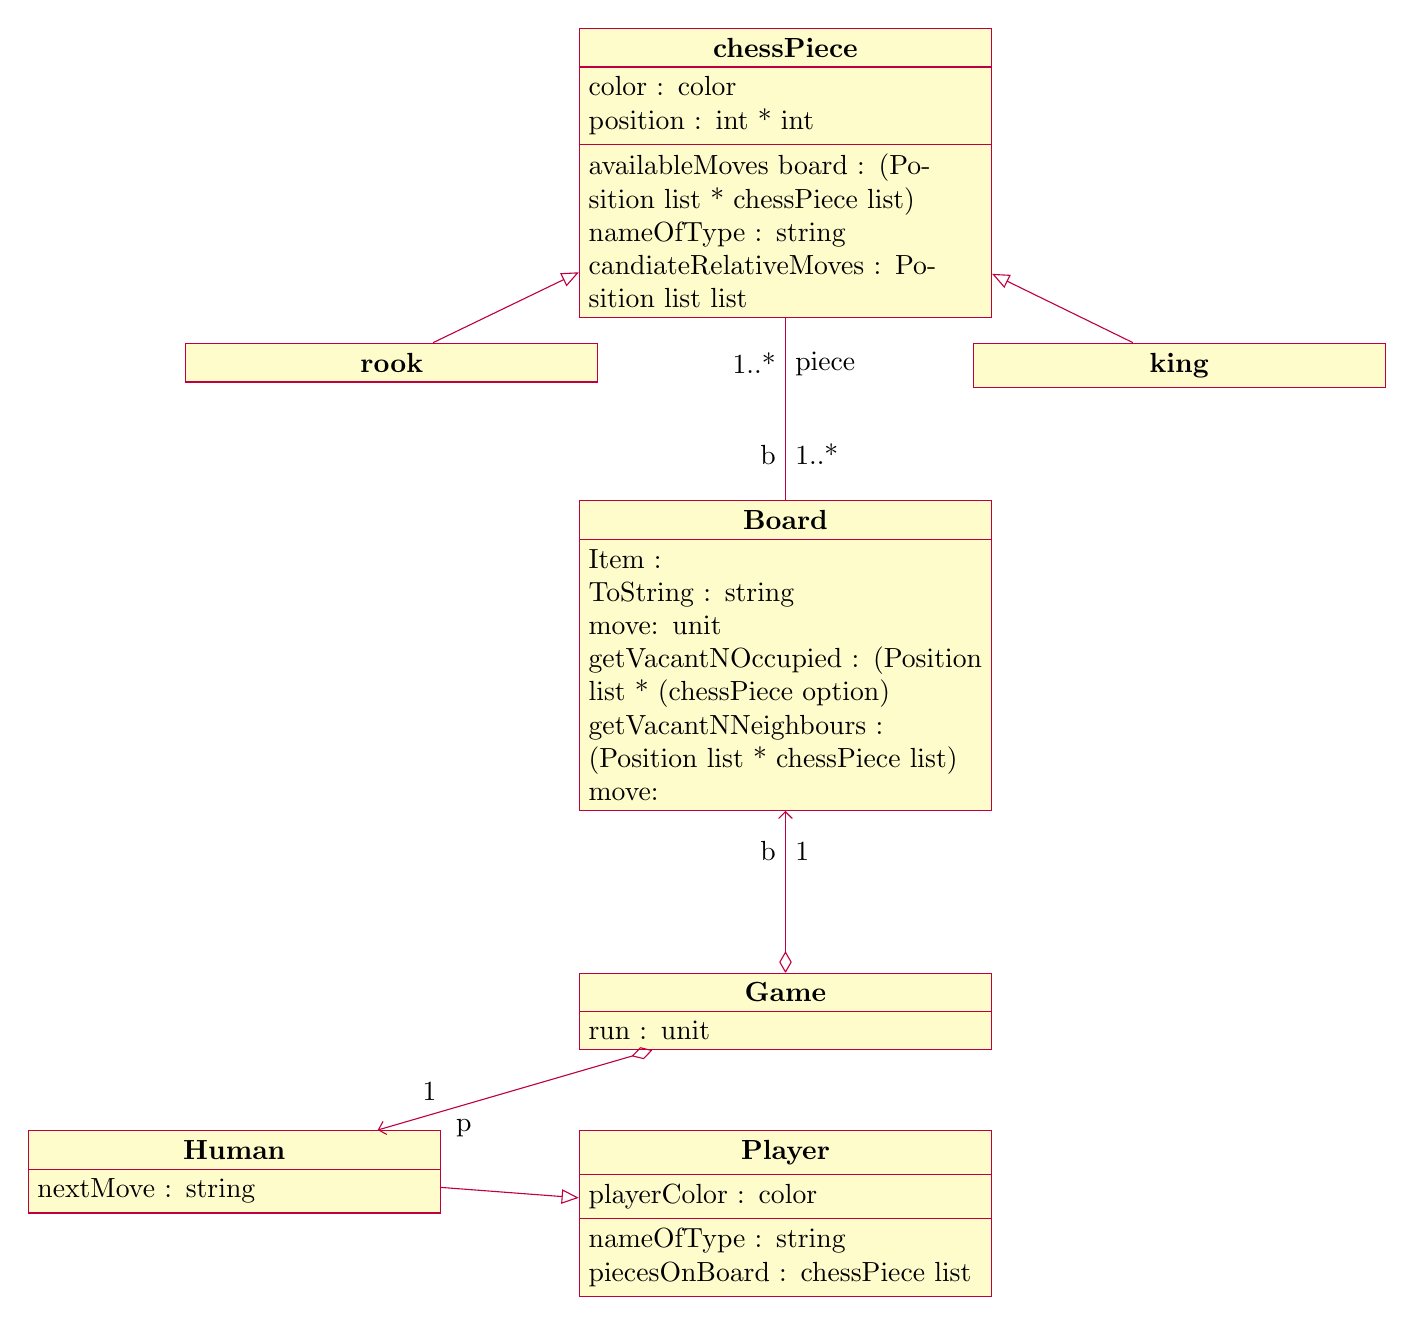
\begin{tikzpicture}
 \begin{class}[text width=5cm]{chessPiece}{0,0}
  \attribute{color : color}
  \attribute{position : int * int}
  \operation{availableMoves board : (Position list * chessPiece list)}
  \operation{nameOfType : string}
  \operation{candiateRelativeMoves : Position list list}
 \end{class}
 \begin{class}[text width=5cm]{rook}{-5,-4}
  \inherit{chessPiece}
 \end{class}
 \begin{class}[text width=5cm]{king}{5,-4}
  \inherit{chessPiece}
 \end{class}
 \begin{class}[text width=5cm]{Board}{0,-6}
  \operation{Item : }
  \operation{ToString : string}
  \operation{move: unit}
  \operation{getVacantNOccupied : (Position list * (chessPiece option)}
  \operation{getVacantNNeighbours : (Position list * chessPiece list)}
  \operation{move: }
 \end{class}
 \association{Board}{b}{1..*}{chessPiece}{1..*}{piece}
 \begin{class}[text width=5cm]{Game}{0,-12}
  \operation{run : unit}
 \end{class}
 \aggregation{Game}{b}{1}{Board}
 \begin{class}[text width=5cm]{Player}{0,-14}
  \attribute{playerColor : color}
  \operation{nameOfType : string}
  \operation{piecesOnBoard : chessPiece list}
 \end{class}
  \begin{class}[text width=5cm]{Human}{-7,-14}
  \inherit{Player}
  \operation{nextMove : string}
 \end{class}
 \aggregation{Game}{p}{1}{Human}
\end{tikzpicture}

\section*{Program description}

From the assignment material we were given a substantial contribution of code, which forms the base for the main functionality of the game.
As mentioned in \textsc{Problem analysis \& design} one of the biggest challenges we faced in getting the code one step closer to a playable game was, to contain the moves available to the king piece.
In its original state, the code given from the assignment allowed the king piece to make moves, which were self-endangering. We therefore had to develop the code, so that this possibility was eliminated.

To do this we developed a function \texttt{riskZone}, that evaluates the piece, which a player tries to move, and given a king piece excludes any "illegal" moves by cross-referencing the $x$ and $y$ coordinate of the target position of the move, with the $x$ and $y$ coordinate of any opponent piece. Then using this to check if there was any duplicates. This made way for creating a list of the coordinates of any opponent piece with an $x$ or $y$ coordinate matching those of the target position. Finally we use this list, to filter the king piece list of possible moves from holding the risky/illegal moves.\\

As the above restriction only applies to the king piece, in regards to the possible moves of the rook piece, we only had to link the pre-developed lists of the valid moves + possible kills of the current piece, into one joined list of possible moves.

\lstinputlisting[language=FSharp, firstline=103, lastline=136]{COPYforReport_chess.fs}

\subsection*{User manual}

\subsubsection*{Getting started}

To start the game follow these steps:
1. Open a terminal
2. Locate the folder 11g\_PernilleIngeChristoffer
3. When inside the folder run the following in the terminal/command: \texttt{bash compileSimpleChess.sh}

If you are using windows or the above instructions does not work please follow these steps:
1. Open a cmd
2. Locate the folder  11g\_PernilleIngeChristoffer
3. When inside the folder compile the application by running the following in the terminal/command prompt:\\
\texttt{fsharpc -a chess.fs -a pieces.fs}\\
\texttt{fsharpc -r chess.dll -r pieces.dll chessApp.fsx}\\
\texttt{mono chessApp.exe}

\subsubsection*{Playing the game}

After compiling the application in the terminal/command prompt the user will have a cleared console displaying only the chess game-board in its initial game state.
By default the game is initialized as a two-player game based on two human players. Unfortunately the current version of the game is not yet developed to handle Human vs. Computer nor Computer vs. Computer.

To play the game, follow the on-screen instructions indicating which player is up. To spice the game up, the user playing as Player Black has red as their piece color, the user playing as Player White has green as their piece color.

To make a move, a player must first type the current position of the piece, which he/she wishes to move, followed by the target position. E.g. “b2 b8” moves the white (green) Rook from its initial position to the far right square of row b (column 8).

The game ends when the king of either one of the players gets killed.

To start a new game re-compile the application.

NOTE: In order to compile the game you must have fsharp installed.


\end{document}